\documentclass[tikz,border=2pt]{standalone}
\usepackage{amsmath,amssymb}
\usepackage{pgfplots}
\pgfplotsset{compat=1.18}

\begin{document}
% X_n -> c in probability: for any fixed tolerance eps the mass outside the band [c-eps, c+eps]
% (shaded tails) goes to 0 as n grows; here X_n ~ N(c, 1/n) for n = 1 and n = 9.
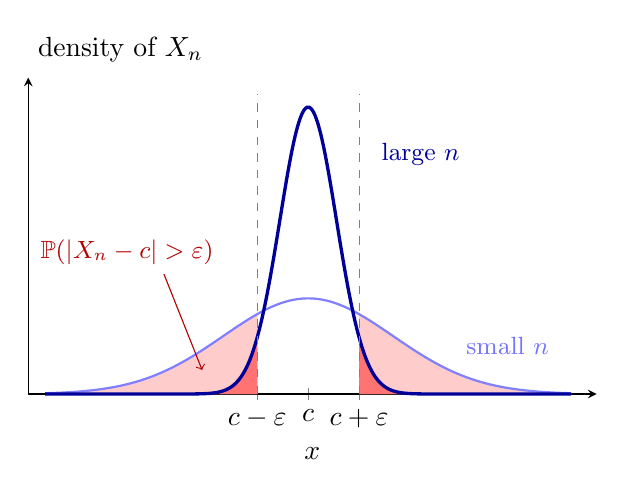
\begin{tikzpicture}
	\begin{axis}[
		axis lines=left, xmin=-3.3, xmax=3.4, ymin=0, ymax=1.32,
		xtick={-0.6,0,0.6}, xticklabels={$c-\varepsilon$,$c$,$c+\varepsilon$}, ytick=\empty,
		xlabel={$x$}, ylabel={density of $X_n$}, ylabel style={rotate=-90, anchor=south west, at={(axis description cs:0,1.02)}},
		samples=200, smooth, width=8.8cm, height=5.6cm, clip=false
		]
		\addplot[fill=red!20, draw=none, domain=-3.1:-0.6] {exp(-x^2/2)/sqrt(2*pi)} \closedcycle;
		\addplot[fill=red!20, draw=none, domain=0.6:3.1] {exp(-x^2/2)/sqrt(2*pi)} \closedcycle;
		\addplot[fill=red!55, draw=none, domain=-3.1:-0.6] {3*exp(-x^2*4.5)/sqrt(2*pi)} \closedcycle;
		\addplot[fill=red!55, draw=none, domain=0.6:3.1] {3*exp(-x^2*4.5)/sqrt(2*pi)} \closedcycle;
		\addplot[blue!50, thick, domain=-3.1:3.1] {exp(-x^2/2)/sqrt(2*pi)};
		\addplot[blue!60!black, very thick, domain=-3.1:3.1] {3*exp(-x^2*4.5)/sqrt(2*pi)};
		\draw[gray, dashed] (axis cs:-0.6,0) -- (axis cs:-0.6,1.25);
		\draw[gray, dashed] (axis cs:0.6,0) -- (axis cs:0.6,1.25);
		\node[blue!55, font=\small, anchor=west] at (axis cs:1.75,0.2) {small $n$};
		\node[blue!60!black, font=\small, anchor=west] at (axis cs:0.75,1.0) {large $n$};
		\node[red!70!black, font=\small, anchor=south east] at (axis cs:-1.0,0.5) {$\mathbb{P}(|X_n-c|>\varepsilon)$};
		\draw[red!70!black, ->] (axis cs:-1.7,0.5) -- (axis cs:-1.25,0.1);
	\end{axis}
	
\end{tikzpicture}
\end{document}
